\documentclass{standalone}
\usepackage{tikz}
\usepackage{ctex,siunitx}
\usepackage{tkz-euclide}
\usepackage{amsmath}
\usetikzlibrary{patterns, calc}
\usetikzlibrary {decorations.pathmorphing, decorations.pathreplacing, decorations.shapes,}
\begin{document}
\small
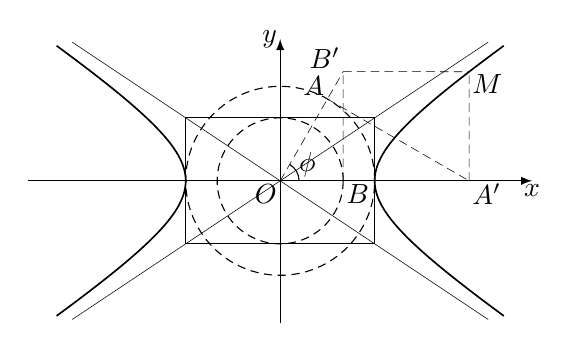
\begin{tikzpicture}[>=latex,scale=0.4,inner sep=1pt]
  \tkzDefPoints{0/0/O,2/0/B,3/2/C1,-3/-2/C2,-3/2/C3,3/-2/C4,2/2/B1}
  \tkzDefPoint(60:3){A}
  \tkzInterLL(O,A)(B,B1)\tkzGetPoint{B'}
  \tkzDefPointBy[rotation=center A angle 90](O)\tkzGetPoint{O'}
  \tkzInterLL(A,O')(O,B)\tkzGetPoint{A'}
  \tkzDefPointBy[translation=from B to B'](A')\tkzGetPoint{M}
  \draw[thin,->](-8,0)--(8,0)node[below]{$x$};
  \draw[thin,->](0,-4.5)--(0,4.5)node[left]{$y$};
  \draw[densely dashed] (O)circle(2)(O)circle(3);
  \draw(C1)rectangle(C2);
  \draw[semithick,domain=-65:65,samples=100] plot ({3/cos(\x)},{2*tan(\x)});
  \draw[semithick,domain=-65:65,samples=100] plot ({-3/cos(\x)},{2*tan(\x)});
  \tkzDrawLines[add=0.6 and 0.6](C1,C2 C3,C4)
  % \draw [semithick] (0,0)circle(1);
  \tkzDrawSegments[densely dashed](O,B' B,B' A,A' A',M B',M)
  % \tkzDrawPoints[fill=black](M)
  \tkzMarkAngle[size=0.6](B,O,A)
  \tkzLabelAngle[pos=1.0](B,O,A){$\phi$}
  % \tkzLabelLine[midway,sloped,above,pos=0.5](A,M){$a$}
  % \tkzLabelLine[midway,sloped,above,pos=0.4](M,B){$b$}
  % \tkzLabelLine[midway,sloped,above,pos=0.7](O,B){$r$}
  \tkzLabelPoints[below right](B,A',M)
  \tkzLabelPoints[below left](O)
  \tkzLabelPoints[above left](A,B')
\end{tikzpicture}
\end{document}